
\section{Arquitectura}
\subsection{Conectores propios}
\subsubsection{Notaci'on}

\begin{itemize}
\item Pipe 
\includegraphics[height=0.6cm]{diagramas/NPIPE} 
\item HC (Holy Connector) 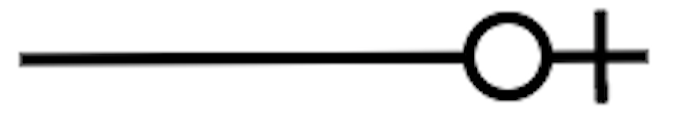
\includegraphics[height=0.5cm]{diagramas/NHC} 
\item AHC (Asynchronous Holy Connector) 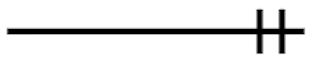
\includegraphics[height=0.5cm]{diagramas/NHCCA}
\item HVC (Holy Video Connector) 
\includegraphics[height=0.5cm]{diagramas/NHVC} 
\item HDC (Holy Data Connector) 
\includegraphics[height=0.5cm]{diagramas/NHDC} 

\end{itemize}

\subsubsection{HC (Holy Connector)}

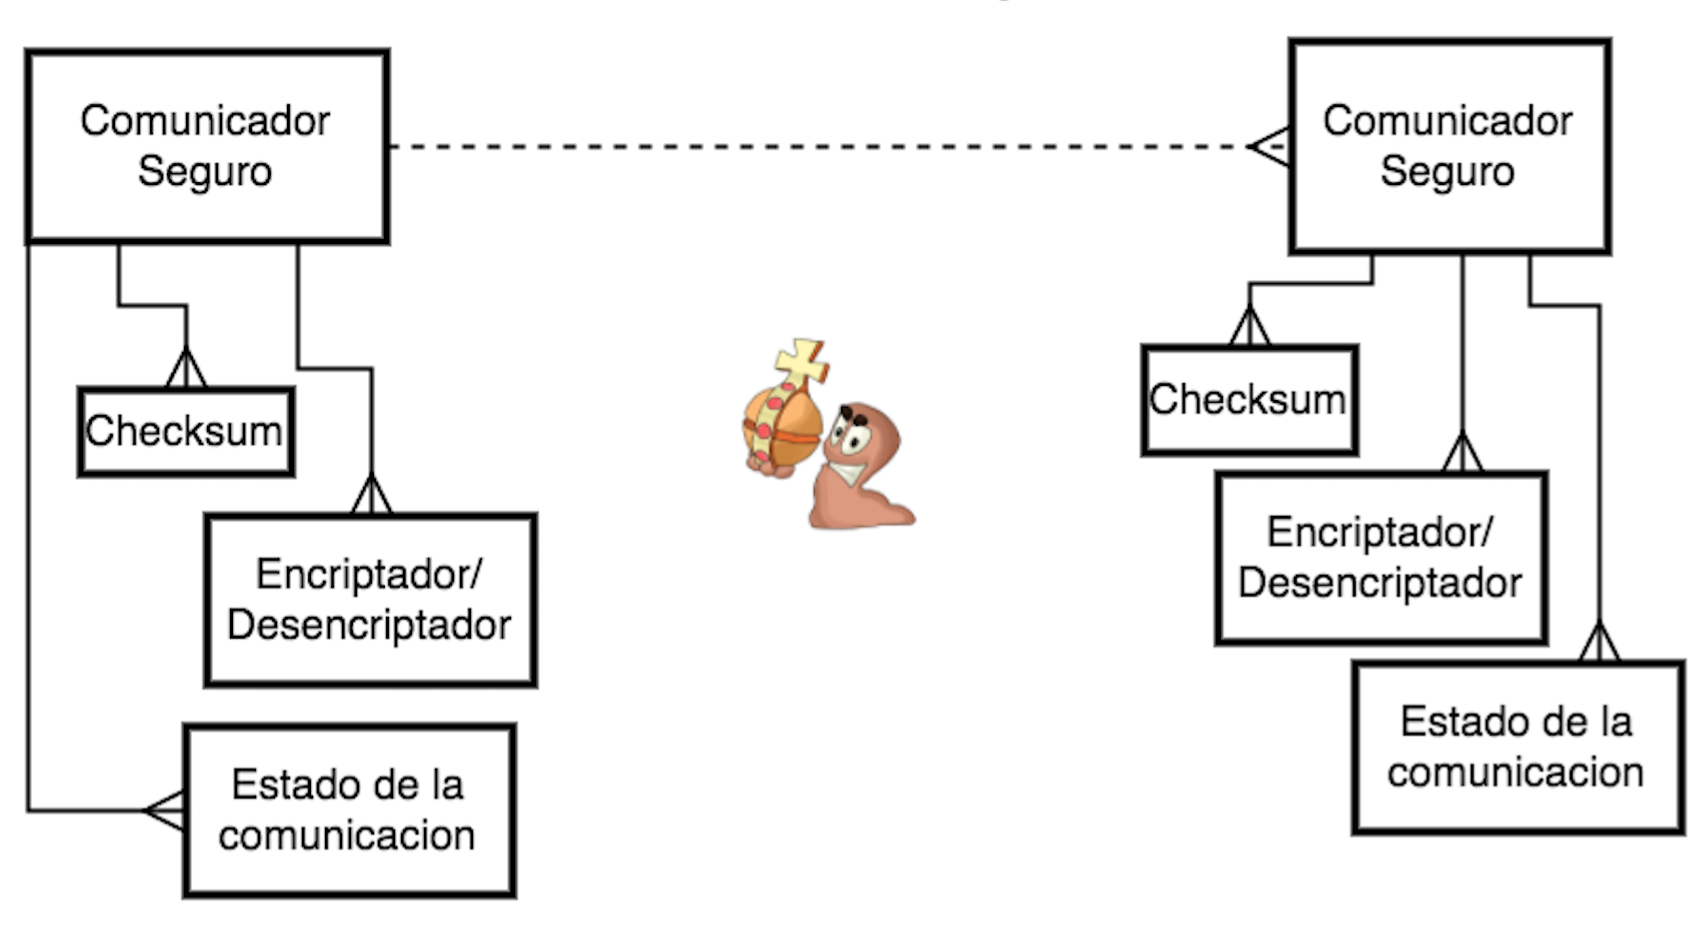
\includegraphics[height=9cm]{diagramas/HC} 

Este conector provee:

\begin{itemize}
	\item \textbf{Seguridad.} Mediante un componente de encriptaci'on y desencriptaci'on de los datos enviados.
	\item \textbf{Integridad.} Mediante un componente de checksum.
	\item \textbf{Confiabilidad de la conexi'on.} Mediante un componente que mantiene el estado de la conexi'on. Por ejemplo, este componente podr'ia implementar el protocolo TCP.
\end{itemize}

Observemos que entre los extremos utilizamos un conector tipo client-server que, asumimos, que se extiende sobre un medio inseguro. Por lo tanto, podemos pensar al Holy Connector como un cliente-server seguro, sobre un medio inseguro.

\subsubsection{AHC (Asynchronous Holy Connector)}

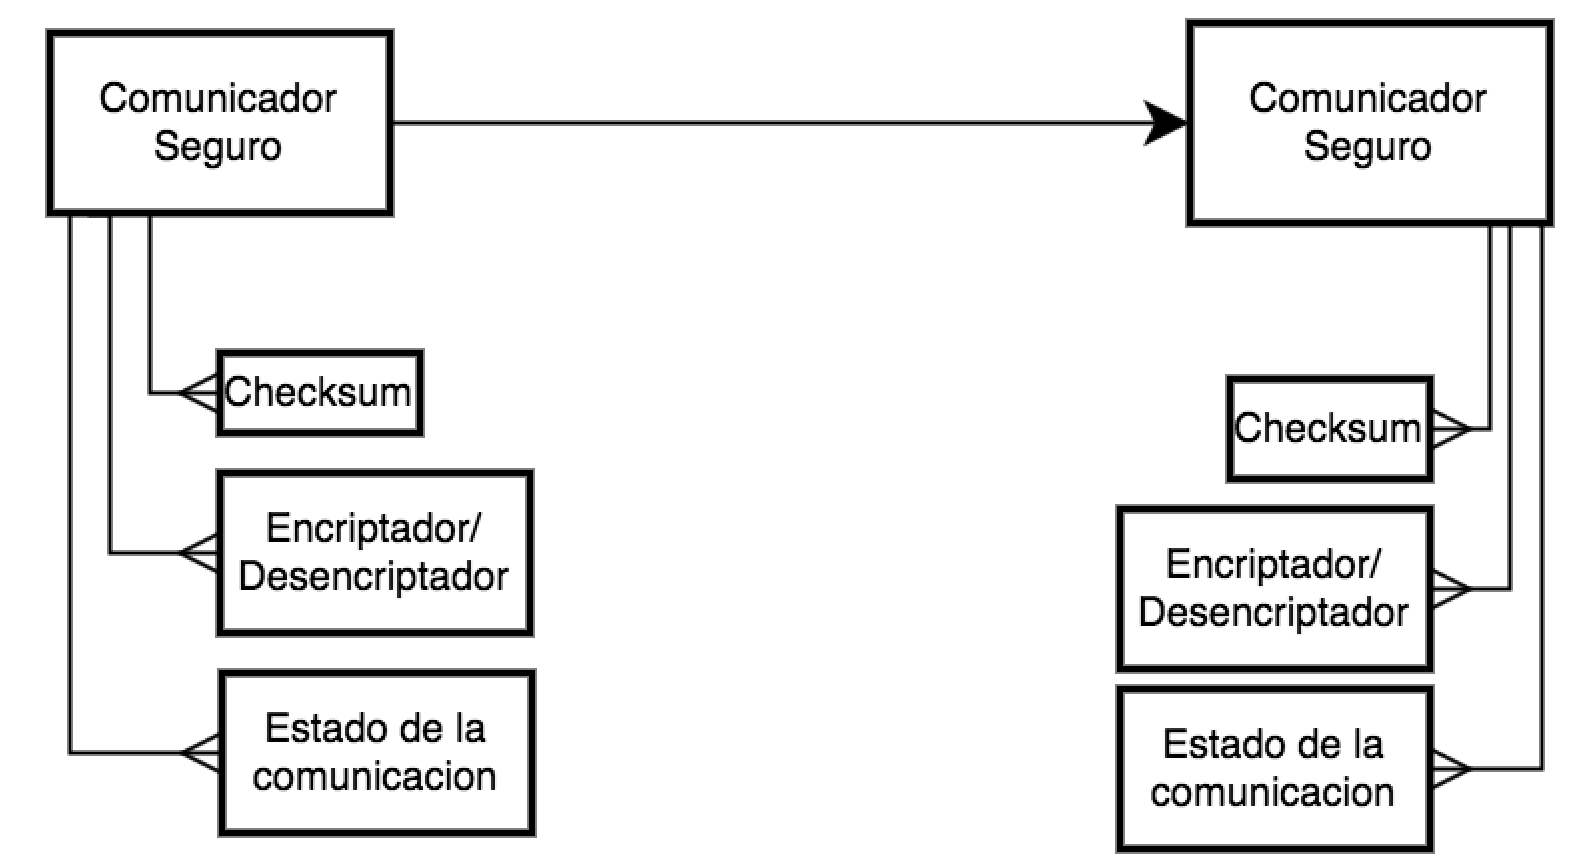
\includegraphics[height=9cm]{diagramas/HCCA} 

Id'entico al Holy Connector, con la diferencia de que en lugar de usar un client-server como conector intermedio, utilizamos un conector de call asincr'onico.

\subsubsection{HVC (Holy Video Connector)}

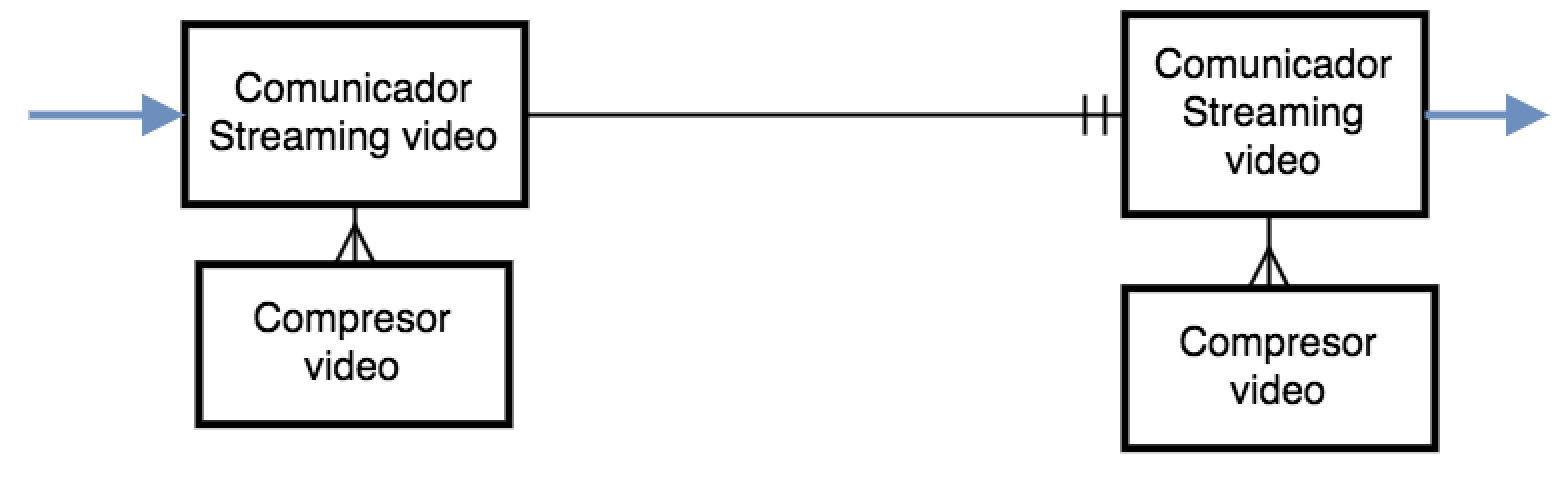
\includegraphics[height=5cm]{diagramas/HVC} 

Contamos en ambos extremos con comunicadores de streaming, que se comunican mediante un Holy Connector. Adicionalmente tenemos, en ambos extremos, compresores adecuados, para que la tasa de cantidad de informaci'on transmitida sea m'as alta.

En ambos extremos tenemos, adem'as, pipes como conectores de entrada y salida. Este buffering permite el env'io y recepci'on de datos flu'ida (evita los tipicos mensajes ``\textbf{buffering...}'').


\subsubsection{HDC (Holy Data Connector)}

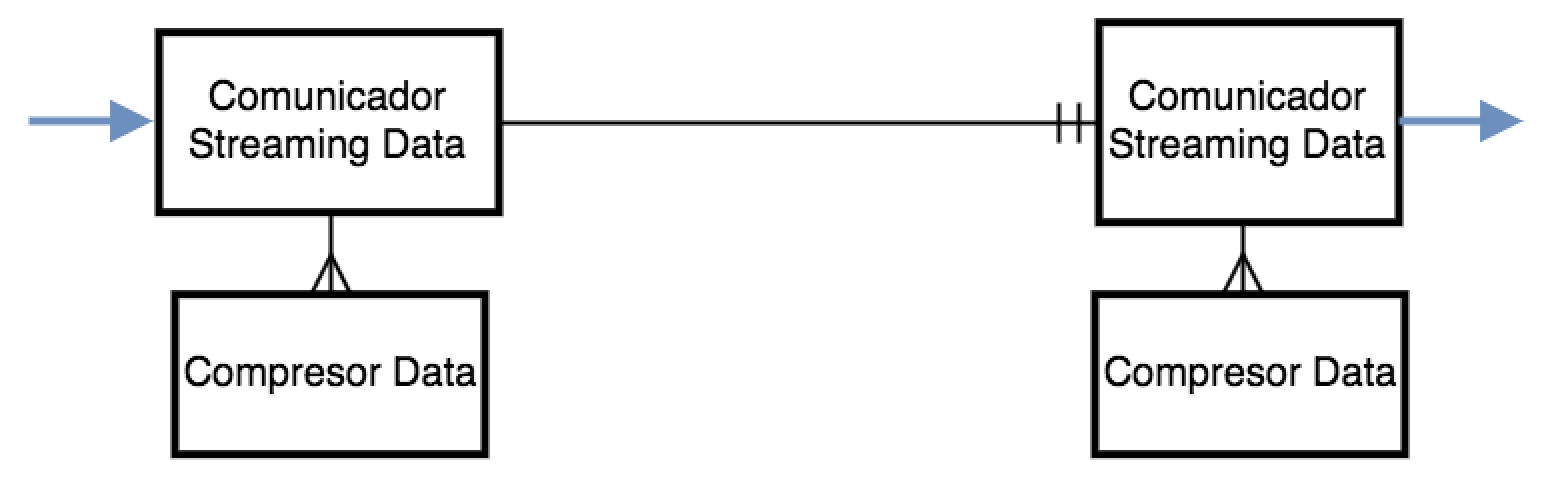
\includegraphics[height=5cm]{diagramas/HDC} 

An'alogo al HVC, pero con compresores adecuados para texto en lugar de video. 

\subsection{Diagrama}

\subsubsection{Descripci'on general}

Para describir la arquitectura, optamos por explicar c'omo se satisface cada una de los requerimientos indicados en el enunciado.

\textit{Lo primero que se pretende es que abarque varios de los deportes colectivos más populares del planeta. Además del ya citado básquet, deberá incorporar a las ligas de fútbol, hockey, rugby, béisbol y fútbol americano que se determine tengan mayor número de seguidores (ej. el fútbol español o la NFL estadounidense), y que se consigan empresas que provean datos en tiempo real de la evolución del partido (tanto del desempeño de los jugadores como del partido en general). Esto último es importante porque además de la simulación de los mismos, ahora también se quiere incorporar un modo de liga de fantasía tradicional.}

Para agregar deportes, lo 'unico que se debe hacer es contratar nuevos servicios de transmisi'on de partidos, agregar nuevos par'ametros del juego (i. e. agregar datos al repositorio de \textit{puntajes por acci'on}), y agregar funcionalidad al \textit{administrador de desaf'ios} para que se puedan crear desaf'ios de 'este nuevo deporte.

Los datos de la evoluci'on del partido provienen de los mismos servicios que nos transmiten partidos reales. Tanto los datos de un partido, como la transmisi'on del mismo nos son transmitidos en conjunto. Ver componente \textit{Servicio de transmisi'on de partido real}.

\textit{En este nuevo modo los ganadores de los desafíos ya no se deciden a través de la simulación directa de los partidos, sino del desempeño de los jugadores en partidos reales en las ligas en cuestión. Por ej. usando el caso del básquet, se podría otorgar 1 punto por cada punto que haga ese jugador en el partido, 1.5 puntos por cada asistencia, 2 por cada bloqueo o robo, -1 por cada pérdida de balón, etc... El equipo que tenga mayor suma, gana el desafío.}

El puntaje que se asigna a cada acci'on de cada deporte es un par'ametro que se encuentra en el repositorio \textit{puntajes por acci'on}.

\textit{Con respecto a los desafíos, ahora pueden incluir un gran número de partidos, no sólo uno. En el caso de este nuevo modo ``liga fantasía tradicional'', podrían incluirse todos los partidos de una fecha determinada de una liga, o un salteado de un conjunto de fechas cualesquiera, o incluso la liga o torneo completo.}

Los desaf'ios son creados por un cliente (un jugador) desde la pantalla de lista de desaf'ios, mediante el m'odulo \textit{creador de desaf'ios}. 'Este le env'ia un pedido al 



\subsubsection{Arquitectura de datacenters}

Nuestro sistema tiene una arquitectura distribuida, basada en datacenters. Un datacenter contiene una gran cantidad de servidores que proveen el servicio de juego. Dentro de un datacenter, los servidores se dividen en conjuntos, y cada conjunto provee servicio a una regi'on distinta. En otras palabras, un datacenter puede proveer servicio a distintas regiones por medio de cierto conjunto de servidores.

Todas las peticiones ingresantes en un datacenter son recibidas y procesadas por una m'aquina de tipo \textit{router}. Un router redirige la petici'on a alg'un servidor de la regi'on correspondiente. Los routers pueden rutear al conjunto de servidores de cualquiera de las regiones servidas en el datacenter. Por ejemplo, podr'ia haber un datacenter en Argentina, que provea el servicio para Argentina, Brasil y Uruguay; en este caso, los routers del datacenter procesan peticiones de las tres regiones.

El siguiente diagrama muestra lo descripto.

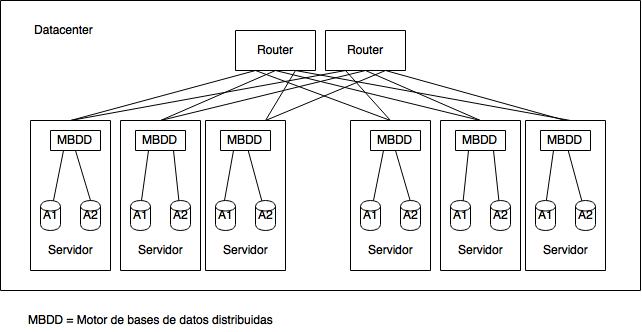
\includegraphics[width=15cm]{diagramas/datacenter.png}

\noindent
El datacenter de la figura tiene dos routers, que procesan pedidos para dos regiones. Cada regi'on se compone de tres servidores. Notar que una de las regiones contiene dos tipos de repositorios, A1 y A2. Estos repositorios aparecen en todos los servidores de la regi'on, debido a que los datos est'an distribuidos sobre todos estos servidores. An'alogamente, los servidores de la otra regi'on, tienen repositorios B1 y B2, distribuidos.

Cada servidor tiene un componente, denominado \textit{agente}. Un agente es la interfaz de todos los repositorios que contiene un servidor, y forman parte del sistema de distribuci'on de datos sobre el conjunto de servidores de una regi'on en un datacenter.

Este esquema de distribuci'on de datos sobre servidores es lo que permite que el sistema sea escalable. Adem'as provee otras bondades como capacidad de replicaci'on de datos, necesario para tener alta disponibilidad. M'as a'un, es posible implementar distribuci'on de datos entre datacenters, haciendo que el conjunto de servidores est'e distribu'ido en m'as de un datacenter. Esto se muestra en la siguiente figura.

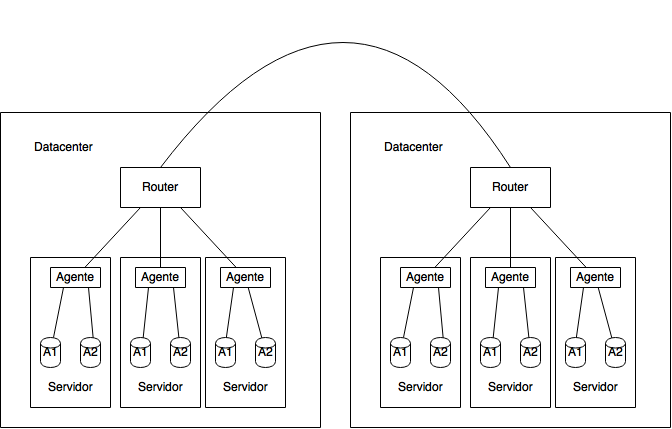
\includegraphics[width=15cm]{diagramas/datacenterx2.png}

\noindent
De esta forma podemos implementar replicaci'on de datos entre datacenters, y as'i si un datacenter se cae, no perdemos datos ni capacidad de proveer servicio a una regi'on.

\subsection{Repositorios}

Los repositorios forman parte de un esquema de almacenamiento de datos distribu'ido. Un repositorio distribu'ido en un datacenter contiene informaci'on sobre la regi'on en la que se encuentra el datacenter.

\begin{itemize}
	\item \textbf{Apuestas por partido.} Contiene las apuestas involucradas en cada partido en ejecuci'on.
	\item \textbf{Partidos pendientes y en ejecucion.} Contiene los partidos (tanto de desaf'io simulaci'on como fantas'ia) que est'an pendientes y en ejecuci'on.
	\item \textbf{Servidores simulando o transmitiendo partido.} Contiene los servidores que est'an simulando o transmitiendo cada partido.
	\item \textbf{Estad'isticas de jugador.} Contiene informaci'on estad'istica, como por ejemplo la cantidad de partidos ganados y perdidos, de cada jugador.
	\item \textbf{Informaci'on de eventos reales.} Contiene toda la informaci'on sobre eventos reales en los que se basan partidos fantas'ia.
	\item \textbf{Usuarios conectados a desaf'io.} Contiene ID e IP de los usuarios actualmente conectados a la sala de un desaf'io.
	\item \textbf{Regiones habilitadas para jugar.} Contiene las regiones a las que se les puede prestar servicio.
	\item \textbf{Regiones habilitadas para transmisi'on de partidos fantas'ia.} Contiene las regiones a las que se les puede transmitir un partido real desde 'esta regi'on.
	\item \textbf{Datos de jugador.} Contiene los datos de un jugador de la regi'on.
	\item \textbf{Estado de partido en ejecuci'on.} Contiene los datos de estado, por ejemplo puntaje de cada equipo, de los partidos que se est'an ejecutando en este momento.
	\item \textbf{Fixtures de desaf'ios.} Contiene los fixtures actualizados de los desaf'ios que a'un no acabaron. En particular, contiene los fixtures de los desaf'ios que a'un no han empezado.
	\item \textbf{Puntaje por acciones.} Contiene informaci'on sobre los par'ametros que se utilizan para puntuar las acciones que ocurren en un partido fantas'ia.
	\item \textbf{Premios por desaf'io.} Contiene los premios (monetarios y no monetarios) que se otorgan a los participantes desaf'ios que a'un no han acabado.
	\item \textbf{M'etodos de pago.} Contiene la informaci'on sobre los servicios de pago que se aceptan en 'esta regi'on.
	\item \textbf{Informaci'on de redes sociales.} Contiene la informaci'on m'as reciente descargada de redes sociales.
	\item \textbf{Publicidades.} Contiene las publicidades m'as recientes recibidas desde los proveedores de publicidad.
\end{itemize}

\subsubsection{Atributos de Calidad vs Arquitectura}
A continuacion listamos todos los atributos de calidad detallados en la seccion anterior y explicamos como hicimos para resolverlo en el diagrama de componentes y conectores.

\begin{itemize}
\item Atributo: El sistema debe evitar que los servidores superen su l'imite de clientes y se caigan.
\item Justificaci'on: Los componentes \textit{router} que reciben las peticiones de un cliente mantienen contadores acerca de la carga de los servidores. Cuando detectan una posible sobrecarga consultan la cantidad de usuarios conectados a los servidores de una regi'on. Lo hacen consultando el repositorio \textit{usuarios conectados a desaf'io}. Si hay sobrecarga, no se responde a las peticiones.

\item Atributo: Desea que haya un esfuerzo por respetar a los países en los que su legislación no permite que directamente se ingrese al sitio.
\item Justificacion: Los \textit{router} que reciban peticiones provenientes de regiones no habilitadas, no ser'an resueltas. Las regiones no habilitadas se consultan en el repositorio \textit{regiones habilitadas para jugar}.

\item Atributo: Se requiere que sea fácil desactivar una cuenta por un tiempo, para ayudar a los adictos en recuperación.
\item Justificacion: Se incluye un m'odulo para desactivar una cuenta, en el programa cliente.

\item Atributo: El simulador debe poder extenderse para soportar reglamentaciones nuevas ya que se espera poder incluir pa'ises adicionales.
\item Justificacion: La modificabilidad el simulador corre por cuenta de los desarolladores del mismo. En el caso del modo fantas'ia, cuya operatoria depende de nuestros desarrolladores, se incluye un repositorio con datos de configuraci'on para los partidos de dicho modo.

\item Atributo: El sistema debe correr en la mayor cantidad de plataformas posible. El sistema debe poder extenderse f'acilmente para incluir nuevas plataformas.
\item Justificacion: La arquitectura del sistema no asume requerimientos de hardware o software (salvo algunos muy b'asicos) sobre el cliente. Para poder soportar todo el abanico de dispositivos, desde aquellos con recursos de hardware y software limitados como aquellos de altas prestaciones, se incluyen dos motores gr'aficos, uno 3D (de altos requerimientos) y otro 2D (de bajos requerimientos). La decisi'on sobre cu'al utilizar se toma en base a los recursos disponibles al momento de la recepci'on de los resultados de la simulaci'on.

\item Atributo: 
\item Justificacion:

\item Atributo: 
\item Justificacion:

\item Atributo: 
\item Justificacion:
\end{itemize}

